\chapter{نمودارهای کلاس طراحی}
در این فصل نمودارهای کلاس طراحی همراه با جزییات آن‌ها آورده شده است. به علت جلوگیری از ناخوانا شدن، از مکانیزم بسته‌بندی
\LTRfootnote{Packaging}
استفاده شده است. در هر بسته چند کلاس مرتبط به همراه ارتباطهایشان با کلاس‌های بیرونی قابل مشاهده است.
\section{بسته پروژه}
\begin{figure}[H]
	\centering
	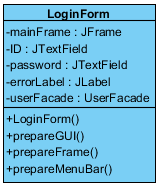
\includegraphics[scale=0.8]{img/des_class/LoginForm}
	\caption{صفحه ورود}
\end{figure}

\section{بسته منبع}
\begin{figure}[H]
	\centering
	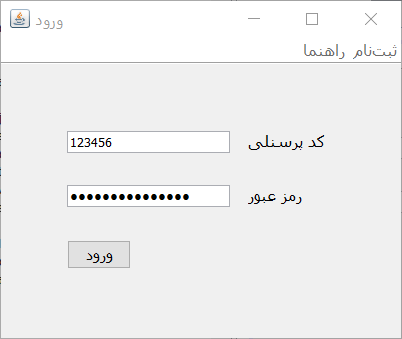
\includegraphics[scale=0.8]{img/prot/LoginForm}
	\caption{صفحه ورود}
\end{figure}

\section{بسته واحد}
\begin{figure}[H]
	\centering
	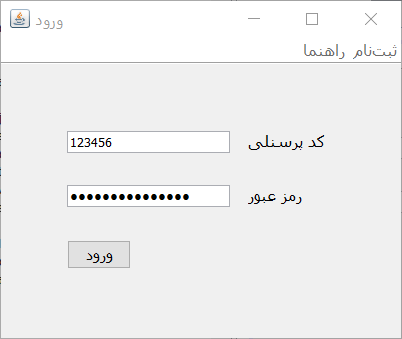
\includegraphics[scale=0.8]{img/prot/LoginForm}
	\caption{صفحه ورود}
\end{figure}

\section{بسته گزارش}
\begin{figure}[H]
	\centering
	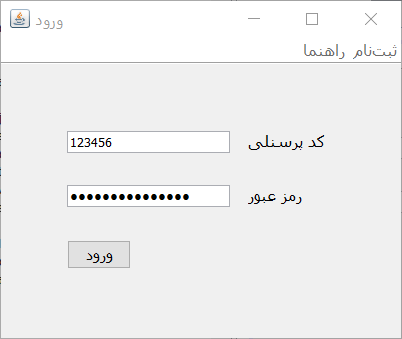
\includegraphics[scale=0.8]{img/prot/LoginForm}
	\caption{صفحه ورود}
\end{figure}

\section{بسته سطح دسترسی}
\begin{figure}[H]
	\centering
	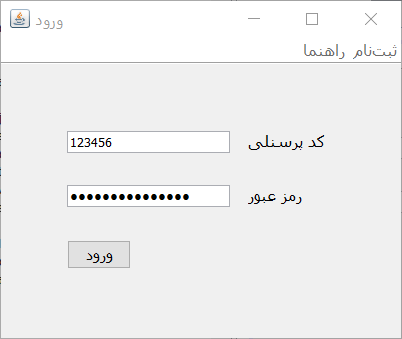
\includegraphics[scale=0.8]{img/prot/LoginForm}
	\caption{صفحه ورود}
\end{figure}

\section{بسته پایگاه‌داده}
\begin{figure}[H]
	\centering
	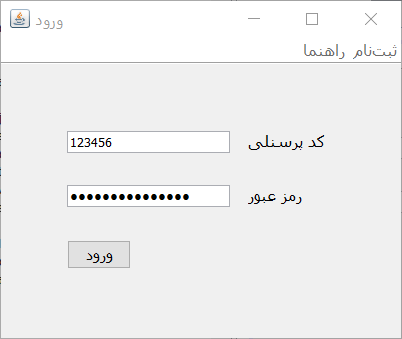
\includegraphics[scale=0.8]{img/prot/LoginForm}
	\caption{صفحه ورود}
\end{figure}

\section{بسته واسط کاربری}
\begin{figure}[H]
	\centering
	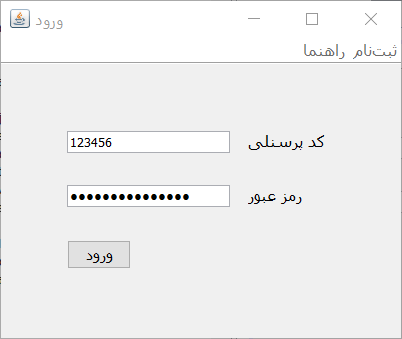
\includegraphics[scale=0.8]{img/prot/LoginForm}
	\caption{صفحه ورود}
\end{figure}
